\section{The Fundamental Theorem of Calculus}
\label{sec:fund-theorem}
% From Section 3.2.
This section contains the most important and most used theorem of calculus, the Fundamental Theorem of Calculus. Discovered independently by Newton and Leibniz in the late 1600s, it establishes the connection between derivatives and integrals, provides a way of easily calculating many integrals, and was a key step in the development of modern mathematics to support the rise of science and technology. Calculus is one of the most significant intellectual structures in the history of human thought, and the Fundamental Theorem of Calculus is a most important brick in that beautiful structure.

\begin{theorem}[The Fundamental Theorem of Calculus]
Let $f(x)$ be a function whose derivative is continuous on an interval $[a, b]$. Then
$$\int_a^b f'(x)\,dx = f(b)-f(a) \enspace .$$
\end{theorem}
This is actually not new for us; we've been using this relationship for some time; we just haven't written it this way. This says what we've said before: the definite integral of a rate from $a$ to $b$ is the net $y$-units, the change in $y$, that accumulate between $x=a$ and $x=b$. Here we've just made it plain that that the rate is a derivative.

Thinking about the relationship this way gives us the key to finding exact answers for some definite integrals. If the integrand is the derivative of some function $f$, then maybe we could simply find $f$ and subtract. That would be easier than approximating with rectangles. Going backwards through the differentiation process will help us evaluate definite integrals.

\begin{example}
Find $f(x)$ if $f'(x)=2x$.

\begin{solution}
Oooh, I know this one. It's $f(x)=x^2+3$. Oh, wait, you were thinking something else? Yes, I guess you're right -- $f(x)=x^2$ works too. So does $f(x)=x^2-\pi$, and $f(x)=x^2+104589.2$. In fact, there are lots of answers.
\end{solution}\end{example}

In fact, there are infinitely many functions that all have the same derivative. And that makes sense – the derivative tells us about the shape of the function, but it doesn't tell about the location. We could shift the graph up or down and the shape wouldn't be affected, so the derivative would be the same.

This leads to one of the trickier definitions – pay careful attention to the articles (the versus an), because they're important.

\begin{definition}[Antiderivatives]
An {\bf antiderivative}\index{Antiderivative} of a function $f(x)$ is any function $F(x)$ where $F'(x)=f(x)$.

The antiderivative of a function $f(x)$ is a whole family of functions, written $F(x)+C$, where $F'(x)=f(x)$ and $C$ represents any constant (i.e., a real number).

The antiderivative of $f(x)$ is also called the {\bf indefinite integral}\index{Indefinite integral}\index{Integral!indefinite} of $f(x)$.

{\bf Notation for the Antiderivative}
The antiderivative of $f$ is written
$$\int f(x)\,dx$$
This notation resembles the definite integral, because the Fundamental Theorem of Calculus says antiderivatives and definite integrals are intimately related. But in this notation, there are no limits of integration.

The $\int$ symbol is still called an {\bf integral sign}; the $dx$  on the end still must be included; you can still think of $\int$ and $dx$  as left and right parentheses. The function $f$ is still called the {\bf integrand}.

{\bf Verb Forms}
We {\bf antidifferentiate}, or {\bf integrate}\index{Integrate}, or {\bf find the indefinite integral} of a function. This process is called {\bf antidifferentiation} or {\bf integration}\index{Integration}.
\end{definition}

There are no small families in the world of antiderivatives: if $f$ has one antiderivative $F$, then $f$ has an infinite number of antiderivatives and every one of them has the form $F(x)+C$.

\begin{example}
Find an antiderivative of $2x$.

\begin{solution}
We can choose any function we like as long as its derivative is $2x$, so we can pick, say, $F(x)=x^2-5.2$.
\end{solution}\end{example}

\begin{example}
Find the antiderivative of $2x$.

\begin{solution}
  Now we need to write the entire family of functions whose derivatives are $2x$. We can use the $\int$ notation:
$$\int 2x\,dx = x^2+C \enspace .$$
(Don't forget the $+C$!)
\end{solution}\end{example}

\begin{example}
Find $\displaystyle\int e^x\,dx$.

\begin{solution}
This is likely one you remember: $e^x$ is its own derivative, so it is also its own antiderivative. The integral sign tells us that we need to include the entire family of functions, so we need that $+C$ on the end:
$$\int e^x\,dx = e^x+C \enspace .$$
\end{solution}\end{example}

\subsection{Antiderivatives Graphically or Numerically}
Another way to think about the Fundamental Theorem of Calculus is to solve the expression for $F(b)$:

\begin{theorem}[The Fundamental Theorem of Calculus (restated)]
$$\int_a^b F'(x)\,dx = F(b)-F(a) \enspace .$$
The definite integral of a derivative from $a$ to $b$ gives the net change in the original function.

$$F(b)=F(a)+\int_a^b F'(x)\,dx$$
The amount we end up is the amount we start with plus the net change in the function.
\end{theorem}
This lets us get values for the antiderivative – as long as we have a starting point, and we know something about the area.

\begin{example}
  \label{ex:5-4-f}
Suppose $F(t)$ has the derivative $f(t)$ shown in Figure \ref{fig:5-4-f}, and suppose that we know $F(0)=5$. Find values for $F(1)$, $F(2)$, $F(3)$, and $F(4)$.
\begin{figure}[!ht]
  \centering
    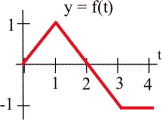
\includegraphics[width=0.3\textwidth]{img/chap5/image036.png}
    \caption{Graph for Example \ref{ex:5-4-f}.}
    \label{fig:5-4-f}
\end{figure}

\begin{solution}
Using the second way to think about the Fundamental Theorem of Calculus, $F(b)=F(a)+\displaystyle\int_a^b F'(x)\,dx$, we can see that $F(1)=F(0)+\int_0^1 f(x)\,dx$. We know the value of $F(0)$, and we can easily find $\displaystyle\int_0^1 f(x)\,dx$ from the graph – it's just the area of a triangle. So
\begin{align*}
F(1) &= 5+0.5=5.5 \\
F(2) &= F(0)+\int_0^2 f(x)\,dx \\
    &= 5+1=6
\end{align*}
Note that we can start from any place of which we know the value; for example, now that we know $F(2)$, we can use that to find
\begin{align*}
F(3) &= F(2)+\int_2^3 f(x)\,dx \\
  &= 6-0.5 = 5.5 \\
F(4) &= F(3)+\int_3^4 f(x)\,dx  \\
  &= 5.5-1=4.5
\end{align*}
\end{solution}\end{example}

\begin{example}
  \label{ex:5-4-F}
The graph of $F'(t)=f(t)$ is shown in Figure \ref{fig:5-4-F} below. Where does $F(t)$ have maximum and minimum values on the interval $[0, 4]$?

\begin{figure}[!ht]
  \centering
    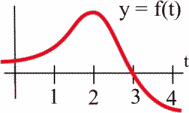
\includegraphics[width=0.3\textwidth]{img/chap5/image037.png}
    \caption{Graph for Example \ref{ex:5-4-F}.}
    \label{fig:5-4-F}
\end{figure}

\begin{solution}
Since $F(b)=F(a)+\displaystyle\int_a^b F'(x)\,dx$, we know that $F$ is increasing as long as the area accumulating under $y = F'(t)=f(t)$ is positive (until $t=3$), and then decreases when the curve dips below the $t$-axis so that negative area starts accumulating. The area between $t=3$ and $t=4$ is much smaller than the positive area that accumulates between 0 and 3, so we know that $F(4)$ must be larger than $F(0)$. The maximum value is when $t=3$; the minimum value is when $t=0$.
\end{solution}\end{example}

Note that this is a different way to look at a problem we already knew how to solve – in Chapter 2, we would have found critical points of $F$, where $f=0$: there's only one, when $t=3$. $f(t)=F'(t)$ goes from positive to negative there, so $F$ has a local max at that point. It's the only critical point, so it must be a global maximum. Then we would look at the values of $F$ at the endpoints to find which was the global minimum.

We can also attempt to sketch a function based on the graph of the derivative.

\begin{example}
  \label{ex:5-4-rocf}
The graph in Figure \ref{fig:5-4-rocf} shows $f'(x)$ – the rate of change of $f(x)$. Use it to sketch a graph of $f(x)$ that satisfies $f(0)=0$.

\begin{figure}[!ht]
  \centering
    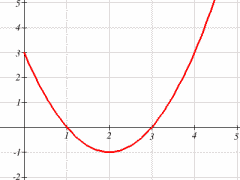
\includegraphics[width=0.3\textwidth]{img/chap5/image038.png}
    \caption{Graph for Example \ref{ex:5-4-rocf}.}
    \label{fig:5-4-rocf}
\end{figure}

\begin{solution}
Recall from Section \ref{sec:sketching} the relationships between the function graph and the derivative graph:
\begin{table}[ht!]
    \centering
    \begin{tabular}{*{5}{l}}
    \toprule
    $f(x)$ &	Increasing &	Decreasing &	Concave Up &	Concave Down	\\
    \midrule
    $f'(x)$	& $+$ & $-$ &	Increasing & Decreasing \\
    \bottomrule
    \end{tabular}
    \caption{The relationship between a function and its derivative.}
    \label{tab:5-derivs}
\end{table}

In the graph shown in Figure \ref{fig:5-4-rocf}, we can see the derivative is positive on the interval $(0, 1)$ and $(3,\infty)$, so the graph of $f$ should be increasing on those intervals. Likewise, $f$ should be decreasing on the interval $(1,3)$.

In the graph, $f'$ is decreasing on the interval $(0, 2)$, so $f$ should be concave down on that interval. Likewise, $f$ should be concave up on the interval $(2,\infty)$.

The derivative itself is not enough information to know where the function $f$ starts, since there are a family of antiderivatives, but in this case we are given a specific point at which to start.

To start the sketch, we might note first the shapes we need:

\begin{figure}[!ht]
  \centering
    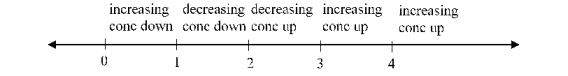
\includegraphics[width=0.7\textwidth]{img/chap5/image067.png}
    \caption{Geometric characteristics of $y=f(x)$.}
    \label{fig:5-4-shapes}
\end{figure}
then sketch the basic shapes:
\begin{figure}[!ht]
  \centering
    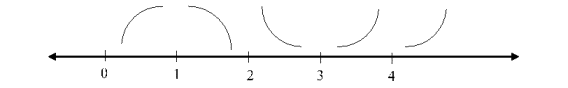
\includegraphics[width=0.7\textwidth]{img/chap5/image068.png}
    \caption{Basic shapes of $y=f(x)$.}
    \label{fig:5-4-curves}
\end{figure}

Now we can attempt to sketch the graph, starting at the point $(0, 0)$. Notice we are very roughly sketching this, as we don't have much information to work with. We can tell, though, from the graph that the area from $x=0$ to $x=1$ is about the same as the area from $x=1$ to $x=3$, so we would expect the net area from $x=0$ to $x=3$ to be close to 0.

\begin{figure}[!ht]
  \centering
    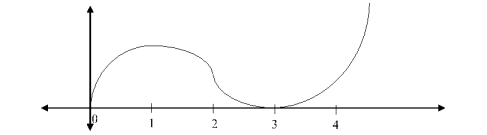
\includegraphics[width=0.5\textwidth]{img/chap5/image069.png}
    \caption{Basic sketch of $y=f(x)$.}
    \label{fig:5-4-sketch}
\end{figure}
It turns out this graph isn't horribly bad. Smoothing it out would give a graph closer to the actual antiderivative graph, shown in Figure \ref{fig:5-4-realsketch}.

\begin{figure}[!ht]
  \centering
    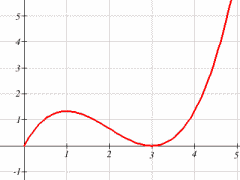
\includegraphics[width=0.4\textwidth]{img/chap5/image039.png}
    \caption{Actual sketch of $y=f(x)$.}
    \label{fig:5-4-realsketch}
\end{figure}
\end{solution}\end{example}

\subsection{Derivative of the Integral}
There is another important connection between the integral and derivative.

\begin{theorem}[The Fundamental Theorem of Calculus (Part 2)]
If
$$A(x)=\int_a^x f(t)\,dt$$
then
$$A'(x)=\frac{d}{dx} \int_a^x f(t)\,dt = f(x) \enspace .$$
I.e., the derivative of the accumulation function is the original function.
\end{theorem}
\begin{example}
  \label{ex:5-4-Fp3}
Let $F(x)=\displaystyle\int_0^x f(t)\,dt$, where $f(x)$ is graphed in Figure \ref{fig:5-4-Fp3}. Estimate $F'(3)$.

\begin{figure}[!ht]
  \centering
    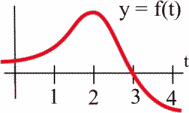
\includegraphics[width=0.3\textwidth]{img/chap5/image037.png}
    \caption{Graph for Example \ref{ex:5-4-Fp3}.}
    \label{fig:5-4-Fp3}
\end{figure}

\begin{solution}
The function $F(x)$ measures the area from $t=0$ to some $t=x$. To estimate $F'(3)$, we want to estimate how much the area is increasing when $t=3$. Since the value of the function $f(t)$ is 0 at $t=3$, the area will not be increasing or decreasing, so we can estimate $F'(3)=0$.

Directly using the Fundamental Theorem of Calculus part 2,
$$F'(x) = \frac{d}{dx} \int_a^xf(t)\,dt = f(x) $$
so
$$F'(x)=f(3)=0 \enspace .$$
\end{solution}\end{example}
